\documentclass{beamer}
\usepackage{beamerthemeshadow}
\usepackage{graphicx}
\usepackage{color}
\usepackage[utf8]{inputenc}
\usepackage{hyperref}
\usepackage[flushleft]{threeparttable}
\usepackage[english,serbian]{babel}
\definecolor{beamer@darkred}{rgb}{0.85,0.1,0.1}
\setbeamercolor{structure}{fg=beamer@darkred}


\title{Tehničko i naučno pisanje}
\subtitle{Kako i zašto funkcioniše blockchain?}
\author{Lazić Jovana, Nikić Ognjen, Nešković Ognjen, Sekešan Pavle}
\institute{Matematički fakultet\\Univerzitet u Beogradu}
\date{
	\footnotesize{Beograd, 2022.}	
}

\begin{document}
\begin{frame}
	\thispagestyle{empty}
	\titlepage
\end{frame}

\addtocounter{framenumber}{-1}

\begin{frame}[fragile]\frametitle{Literatura}
	\begin{itemize}
		\item G. Wood et al., “Ethereum: A secure decentralised generalised transaction ledger,” Ethereum project yellow paper, vol. 151, no. 2014, pp. 1-2, 2014.
		\item S. Nakamoto, “Bitcoin: A peer-to-peer electronic cash system,” Decentralized Business Review, p. 21260, 2008.
		\item H. S. Shin, “Chapter V Cryptocurrencies: looking beyond the hype,”BIS 2018 Annual Economic Report, 2018.
		\item V. Buterin, “A next-generation smart contract and decentralized application platform,” white paper, vol. 3, 2014.
	\end{itemize}
\end{frame}

\begin{frame}
	\frametitle{Pregled} % Table of contents slide, comment this block out to remove it
	\tableofcontents[hidesubsections] 
\end{frame}

\section{Uvod}

\begin{frame}[fragile]\frametitle{Autentičnost dokumenata i konsenzus}
	\begin{itemize}
		\item Kako da znamo da je neko zaista napravio neki dokument?
		\begin{itemize}
			\item U stvarnosti: Potpisi, pečati, hologrami, centralni autoriteti 
			\item U digitalnom svetu: Digitalni potpisi (pomoću asimetrične kriptografije) 
		\end{itemize}
		\item Kako postići konsenzus kada svi ne sarađuju ili se poruke mogu izgubiti ili izmeniti (problem vizantijskih generala)?
		\begin{itemize}
			\item Algoritam za postizanje konsenzusa - na primer prihvatanje odluke koju donese 51\%
			\item U digitalnom svetu - kako obezbediti da svako dobije jedan glas?
		\end{itemize}

	\end{itemize}
\end{frame}

\begin{frame}[fragile]\frametitle{Utvrđivanje hronologije}
	\begin{itemize}
		\item Kako utvrditi hronologiju izmena ili objavljivanja podataka?
		\begin{itemize}
			\item U stvarnosti: centralni autoritet u koji svi imaju poverenje
			\item U digitalnom svetu: Ulančavanje kriptografskih heš funkcija
		\end{itemize}
		\item Kada se ove ova tri problema reše moguće je napraviti javan, verodostojan skup podataka.
	\end{itemize}
\end{frame}


\section{Kriptografske osnove}

\begin{frame}[fragile]\frametitle{Kriptografske heš funkcije - osobine}
	
\end{frame}

\begin{frame}[fragile]\frametitle{Kriptografske heš funkcije - algoritam}
	
\end{frame}

\begin{frame}[fragile]\frametitle{Asimetrična kriptografija}
	
\end{frame}


\section{Blokčejn}

\begin{frame}[fragile]\frametitle{Struktura blokčejna}
	\begin{figure}[H]
		\includegraphics[scale=0.25]{bitcoin_blockchain_diagram.pdf}
	\end{figure}
	\begin{itemize}
		\item Blokovi su manje grupe izmena na skupu podataka (npr. kod Bitkojna - transakcije)
		\item Blokovi su ulančani pomoću heš funkcija
	\end{itemize}
\end{frame}

\begin{frame}[fragile]\frametitle{Blokovi}
	\begin{itemize}
		\item Uz svaki blok se čuva heš koji se dobija tako što se heširaju zajedno podaci iz trenutnog bloka i heš vrednost prethodnog bloka.
		\item Primetimo da je ovako nemoguće izmeniti neki blok bez toga da izmenimo sve blokove nakon njega.
		\item Ovako je utvrđena hronologija izmena
	\end{itemize}
\end{frame}

\begin{frame}[fragile]\frametitle{Decentralizacija}
	\begin{itemize}
		\item Kako utvrditi koji lanac je ispravan?
		\begin{itemize}
			\item Algoritam za postizanje konsenzusa, proof of work, proof of stake...
		\end{itemize}
		\item Kako verifikovati da je neko odobrio neku izmenu?
		\begin{itemize}
			\item Digitalni potpisi
		\end{itemize}
		\item Ako se dva bloka kreiraju u različito vreme - fork:
		\begin{figure}[H]
			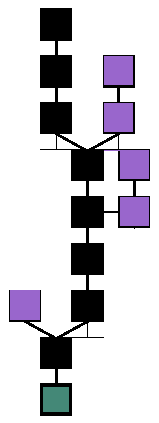
\includegraphics[scale=0.7,angle=-90,origin=c]{blockchain_fork.pdf}
		\end{figure}
	\end{itemize}
\end{frame}


\section{Primene}

\begin{frame}[fragile]\frametitle{Kriptovalute}
	
\end{frame}

\begin{frame}[fragile]\frametitle{Pametni ugovori}
	
\end{frame}

\begin{frame}[fragile]\frametitle{??}
	
\end{frame}


\section{Zaključak}

\begin{frame}[fragile]\frametitle{Zaključak}
	
\end{frame}

\end{document}